\documentclass[UTF8,a4paper,10pt]{ctexart}
\usepackage[left=2.50cm, right=2.50cm, top=2.50cm, bottom=2.50cm]{geometry}
%页边距
\CTEXsetup[format={\Large\bfseries}]{section} %设置章标题居左

%%%%%%%%%%%%%%%%%%%%%%%
% -- text font --
% compile using Xelatex
%%%%%%%%%%%%%%%%%%%%%%%
% -- 中文字体 --
%\setmainfont{Microsoft YaHei}  % 微软雅黑
%\setmainfont{YouYuan}  % 幼圆    
%\setmainfont{NSimSun}  % 新宋体
%\setmainfont{KaiTi}    % 楷体
%\setmainfont{SimSun}   % 宋体
%\setmainfont{SimHei}   % 黑体
% -- 英文字体 --
%\usepackage{times}
%\usepackage{mathpazo}
%\usepackage{fourier}
%\usepackage{charter}

%\usepackage{helvet}

\usepackage{amsmath, amsfonts, amssymb} % math equations, symbols
\usepackage[english]{babel}
\usepackage{color}	% color content
\usepackage{graphicx}	% import figures
\usepackage{url}	% hyperlinks
\usepackage{bm} 	% bold type for equations
\usepackage{multirow}
\usepackage{booktabs}
\usepackage{epstopdf}
\usepackage{epsfig}
\usepackage{algorithm}
\usepackage{algorithmic}
\usepackage{listings}
\usepackage{xcolor}
\usepackage{booktabs}
\usepackage{zhnumber}
\usepackage{longtable}
\usepackage{subfigure}
\usepackage{float}
\usepackage{caption}
\usepackage{subfigure}
\renewcommand\thesection{\zhnum{section}}
\renewcommand \thesubsection {\arabic{section}}
\renewcommand{\algorithmicrequire}{ \textbf{Input:}}
% use Input in the format of Algorithm  
\renewcommand{\algorithmicensure}{ \textbf{Initialize:}}
% use Initialize in the format of Algorithm  
\renewcommand{\algorithmicreturn}{ \textbf{Output:}}
% use Output in the format of Algorithm  
%%%%%%%%%%%%%%%%%%
\usepackage{listings}
\usepackage{color}
\definecolor{dkgreen}{rgb}{0,0.6,0}
\definecolor{gray}{rgb}{0.5,0.5,0.5}
\definecolor{mauve}{rgb}{0.58,0,0.82}
\lstset{frame=tb,
  language=Python,
  aboveskip=3mm,
  belowskip=3mm,
  showstringspaces=false,
  columns=flexible,
  basicstyle={\small\ttfamily},
  numbers=left,%设置行号位置none不显示行号
  %numberstyle=\tiny\courier, %设置行号大小
  numberstyle=\tiny\color{gray},
  keywordstyle=\color{blue},
  commentstyle=\color{dkgreen},
  stringstyle=\color{mauve},
  breaklines=true,
  breakatwhitespace=true,
  escapeinside=``,%逃逸字符(1左面的键),用于显示中文例如在代码中`中文...`
  tabsize=4,
  extendedchars=false %解决代码跨页时,章节标题,页眉等汉字不显示的问题
}

%%%%%%%%%%%%%%%%%%%%%%%%%%%%
\usepackage{fancyhdr} %设置页眉、页脚
\pagestyle{fancy}
\lhead{}
\chead{}
%\rhead{\includegraphics[width=1.2cm]{fig/ZJU_BLUE.eps}}
\lfoot{}
\cfoot{}
\rfoot{}
\fancyfoot[RE,RO]{~\thepage~}

\fancyhead[RE,RO]{计算物理导论 \quad 2022春季学期 \quad 作业4  \quad 何翼成}

%%%%%%%%%%%%%%%%%%%%%%%
%  设置水印
%%%%%%%%%%%%%%%%%%%%%%%
%\usepackage{draftwatermark}         % 所有页加水印
%\usepackage[firstpage]{draftwatermark} % 只有第一页加水印
% \SetWatermarkText{Water-Mark}           % 设置水印内容
% \SetWatermarkText{\includegraphics{fig/ZJDX-WaterMark.eps}}         % 设置水印logo
% \SetWatermarkLightness{0.9}             % 设置水印透明度 0-1
% \SetWatermarkScale{1}                   % 设置水印大小 0-1    

\usepackage{hyperref} %bookmarks
\hypersetup{colorlinks, bookmarks, unicode} %unicode

\title{\textbf{以不同初值出发求解复方程的根}}
\author{ 何翼成 \thanks{学号:520072910043; \newline
    邮箱地址:heyicheng@sjtu. edu. cn} }
\date{\today}

\begin{document}
\maketitle

%\begin{abstract}
%这是一篇中文小论文。这个部分用来写摘要。摘要的章标题默认是英文,还没找到改成中文的方法:(
%\end{abstract}

\section{题目与分析}
从不同初值$z_{0}$出发,用牛顿法求解复方程$z^{4}=1$。那么可以设方程
$f(z)=z^{4}-1$,求解其复数域内的零点。由于是使用牛顿迭代法,即
$z_{n}=z{n-1}-\frac{f(z_{n-1})}{f^{'}(z_{n-1})}$,那么即可使用
matlab中的meshgrid()函数将某个区间内的复数扫描后代入式子中,并且进行
上式描述的迭代,满足一定关系后即可停止并且记录得到的结果。
%\section*{单摆的非线性振动}

\section{代码编写与运行}
题目中对于扫描区域以及扫描的精度有着不同的要求,但是总体上的思路和代码都是可以沿用的。
所以可以编写一个总体的方程,在不同的题目要求下代入不同的初始值即可。\newline
值得注意的是,某些区域进行迭代时得到的结果并非收敛的,所以在编写时额外加入了筛选函数,
将所有发散值都改为统一值,不仅有利于图像的完整,也有利于对得到的结果进行分析。\newline

\subsubsection{总体函数代码展示}
%代码展示的源代码
~\\
\lstset{language=matlab}
\begin{lstlisting}
  function newtonmethod(R,I)
  [rr,ii]=meshgrid(R,I);
  Val_1=zeros(length(R),length(I));
  Val_2=Val_1;
  z_0=rr+ii*1i;
  Val_1=z_0;
  for m=1:length(R)
      for n=1:length(I)
          for i=1:10000
          Val_2(m,n)=Val_1(m,n)-(Val_1(m,n)^4-1)/(4*Val_1(m,n)^3);
          Val_1(m,n)=Val_2(m,n);
          if abs(Val_1(m,n)-Val_2(m,n))<10^(-15)
              break
          end
          end
      end
  end
  for m=1:length(R)
      for n=1:length(I)
          if abs(real(Val_1(m,n)))>1||abs(imag(Val_1(m,n)))>1
              Val_1(m,n)=1.1+1.1*i;
              %对发散值统一取值为1.1+1.1*i,避免对颜色分配造成影响
          end
      end
  end
  t1=real(Val_1);
  t2=imag(Val_1);
  %图一分析实部分布
  figure(1)
  surf(rr,ii,t1)
  axis([R(1) R(end) I(1) I(end) -2 2])
  xlabel('初值实部'),ylabel('初值虚部'),zlabel('收敛值实部')
  colorbar
  %图二分析虚部分布
  figure(2)
  surf(rr,ii,t2)
  axis([R(1) R(end) I(1) I(end) -2 2])
  xlabel('初值实部'),ylabel('初值虚部'),zlabel('收敛值虚部')
  colorbar
  %图三分析整体趋势
  figure(3)
  quiver(rr,ii,t1,t2)
  xlim([R(1) R(end)])
  ylim([I(1) I(end)])
  hold on
  streamslice(rr,ii,t1,t2)
  xlim([R(1) R(end)])
  ylim([I(1) I(end)])
  end
\end{lstlisting}

\subsubsection{函数代码解析}
该函数的大体思路是将不同区域的初值进行代入迭代之后得到了结果,
然而这个值可能收敛也有可能不收敛。在这里为了对计算后的结果进行比较,
这里用了三张图进行不同程度的描述,即:\newline
1)迭代计算后的实部分布图象;\newline
2)迭代计算后的虚部分布图象;\newline
3)利用向量分布图和流线图分析迭代计算后的结果的趋势图像\newline
限于知识水平,在这里没有采用使用颜色对结果进行区分,所以只能使用matlab默认
的colormap功能进行简单的着色。\newline
那么牛顿迭代法的代码已经完毕,就可以代入初值进行分析。

\section{[-1,1]\times [-1,1],d=0.01}
\subsubsection{代码展示}
~\\
\lstset{language=matlab}
\begin{lstlisting}
  %%
clear;clc;
R=-1:0.01:1;
I=-1:0.01:1;
newtonmethod(R,I)
\end{lstlisting}
\subsubsection{结果分析}
%%以下为并列图所用到的模板
\newline
\begin{figure}[htbp]
  \centering
  \subfigure[]
  {
   \begin{minipage}{7cm}
    \centering
    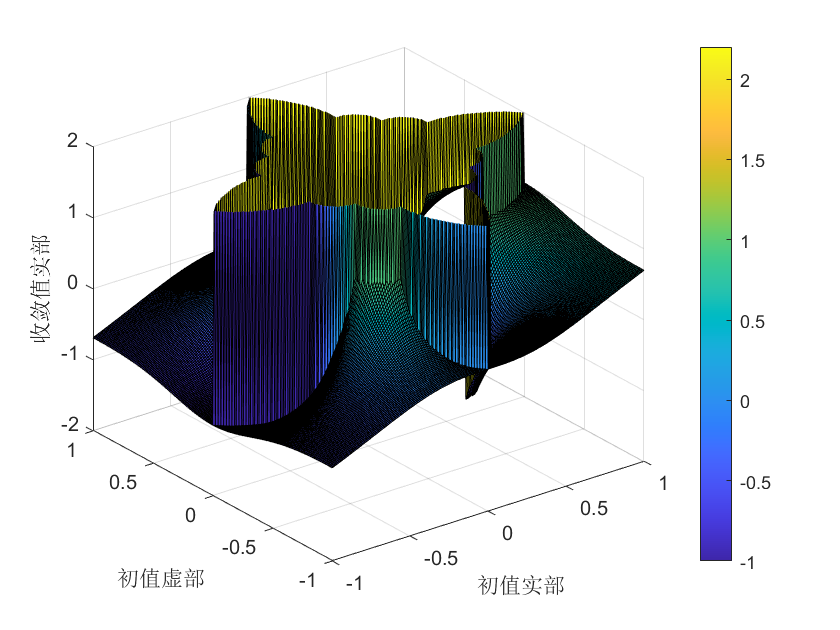
\includegraphics[scale=0.3]{pictures/1_1_1.png}
   \end{minipage}
  }
     \subfigure[]
     {
      \begin{minipage}{7cm}
       \centering
       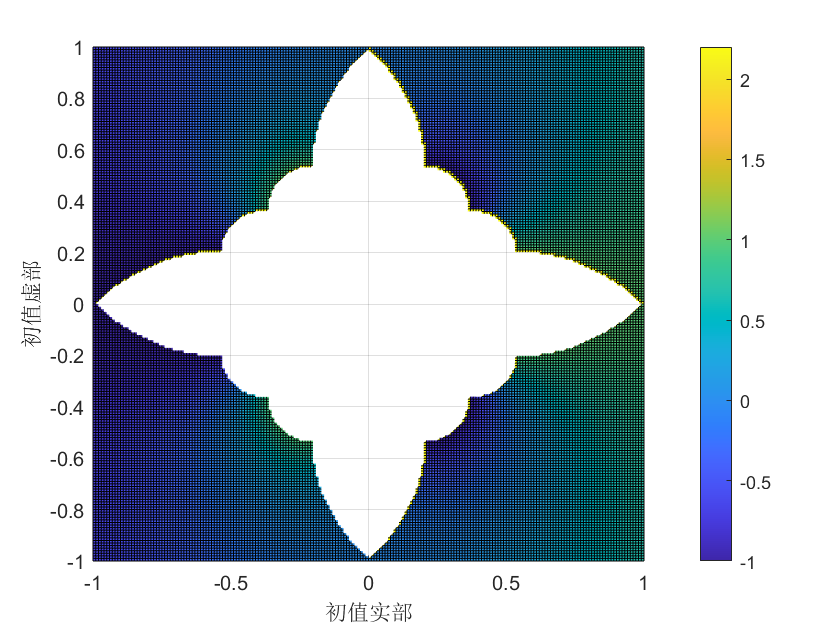
\includegraphics[scale=0.3]{pictures/1_1_2.png}
      \end{minipage}
     }
 \caption{实部总体图(a)和俯视图(b)}}
 \label{1_1}
\end{figure}

\newline
 \begin{figure}[htbp]
  \centering
  \subfigure[]
  {
   \begin{minipage}{7cm}
    \centering
    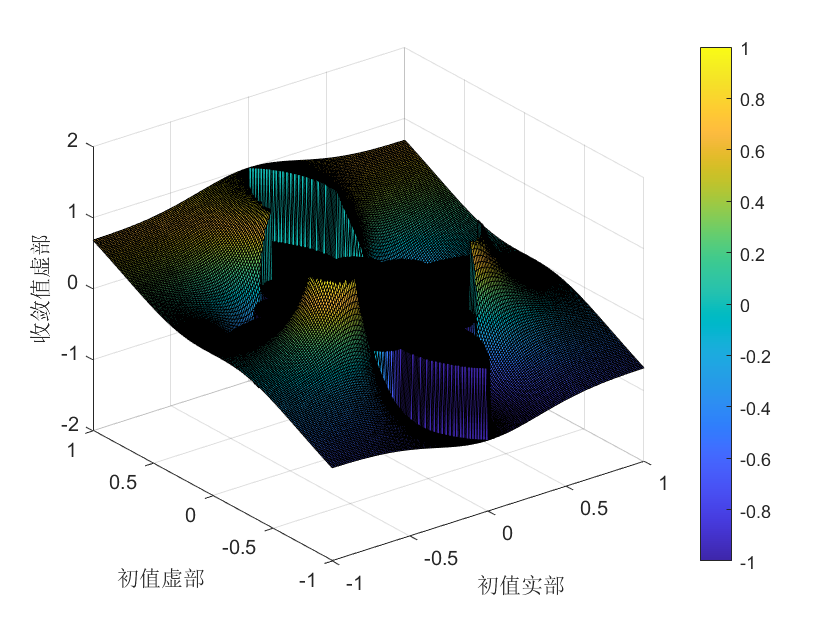
\includegraphics[scale=0.3]{pictures/1_2_1.png}
   \end{minipage}
  }
     \subfigure[]
     {
      \begin{minipage}{7cm}
       \centering
       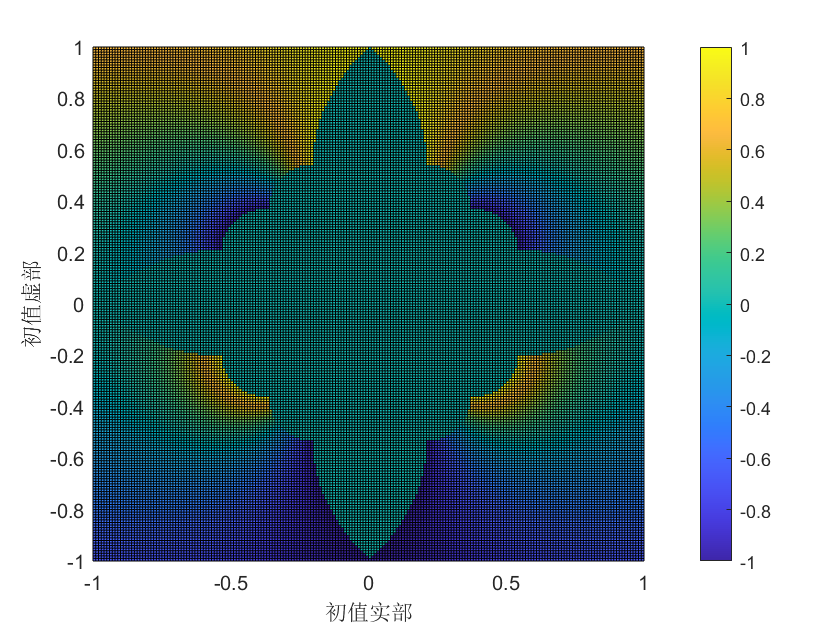
\includegraphics[scale=0.3]{pictures/1_2_2.png}
      \end{minipage}
     }
 \caption{虚部总体图(a)和俯视图(b)}}
 \label{1_2}
 \end{figure}

 \newline
	\begin{figure}[!htbp]
		\centering
		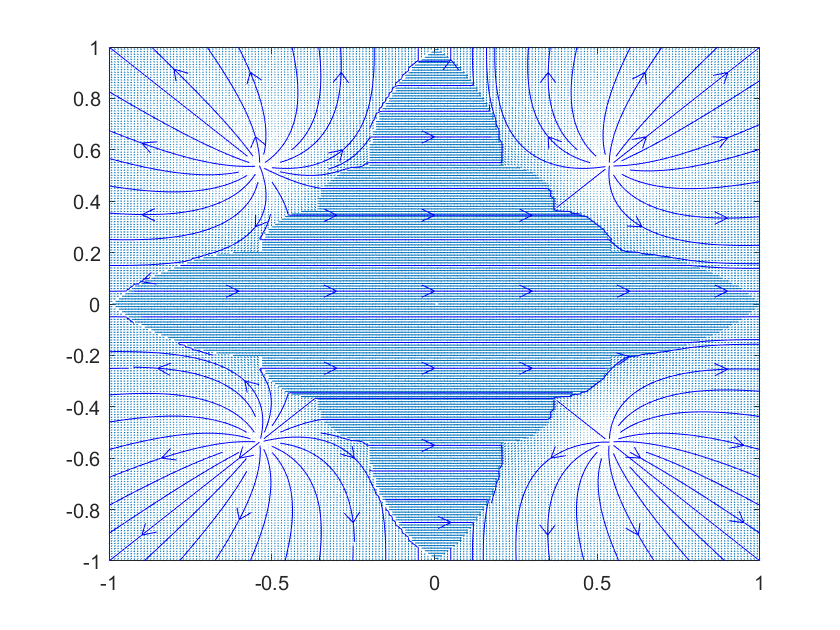
\includegraphics[width=1\textwidth,height=1\textwidth]{pictures/1_3.png}
		\caption{总体趋势图} \label{1_3}
	\end{figure}

\section{[0.4,0.6]\times [0.4,0.6],d=0.001}
\subsubsection{代码展示}
~\\
\lstset{language=matlab}
\begin{lstlisting}
  %%
%从不同初值z_{0}出发,用牛顿法求解复方程z^4=1的根
clear;clc;
R=0.4:0.001:0.6;
I=0.4:0.001:0.6;
newtonmethod(R,I)
\end{lstlisting}
\subsubsection{结果分析}
\newline
\begin{figure}[htbp]
  \centering
  \subfigure[]
  {
   \begin{minipage}{7cm}
    \centering
    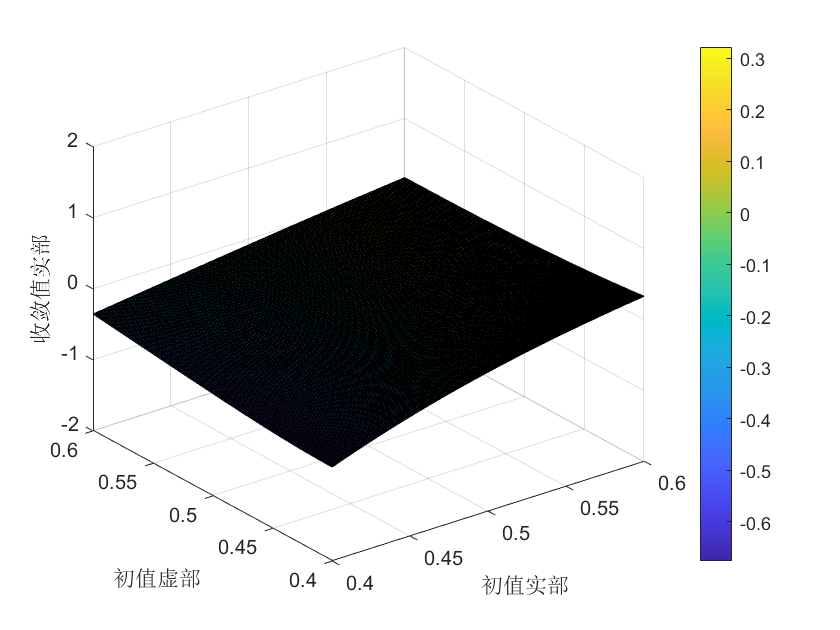
\includegraphics[scale=0.3]{pictures/2_1_1.png}
   \end{minipage}
  }
     \subfigure[]
     {
      \begin{minipage}{7cm}
       \centering
       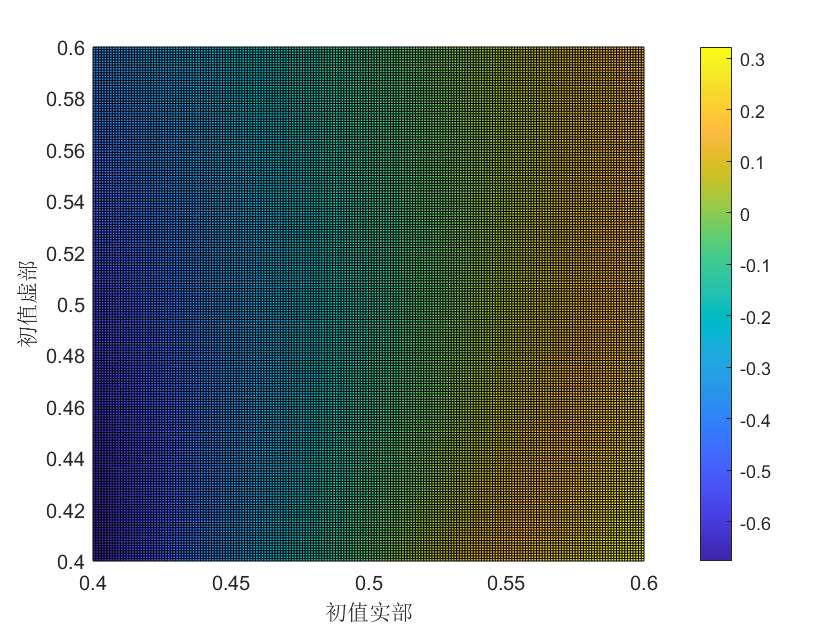
\includegraphics[scale=0.3]{pictures/2_1_2.png}
      \end{minipage}
     }
 \caption{实部总体图(a)和俯视图(b)}}
 \label{2_1}
\end{figure}

\newline
 \begin{figure}[htbp]
  \centering
  \subfigure[]
  {
   \begin{minipage}{7cm}
    \centering
    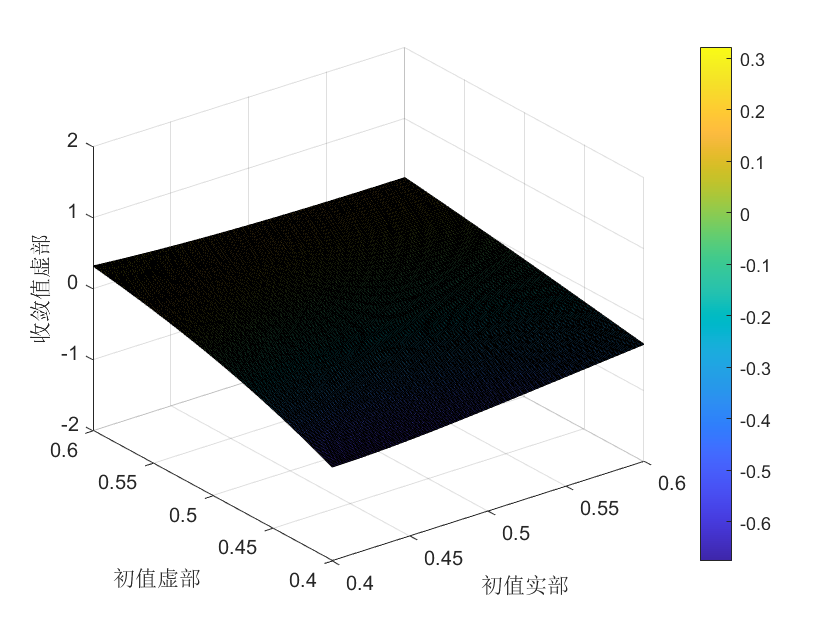
\includegraphics[scale=0.3]{pictures/2_2_1.png}
   \end{minipage}
  }
     \subfigure[]
     {
      \begin{minipage}{7cm}
       \centering
       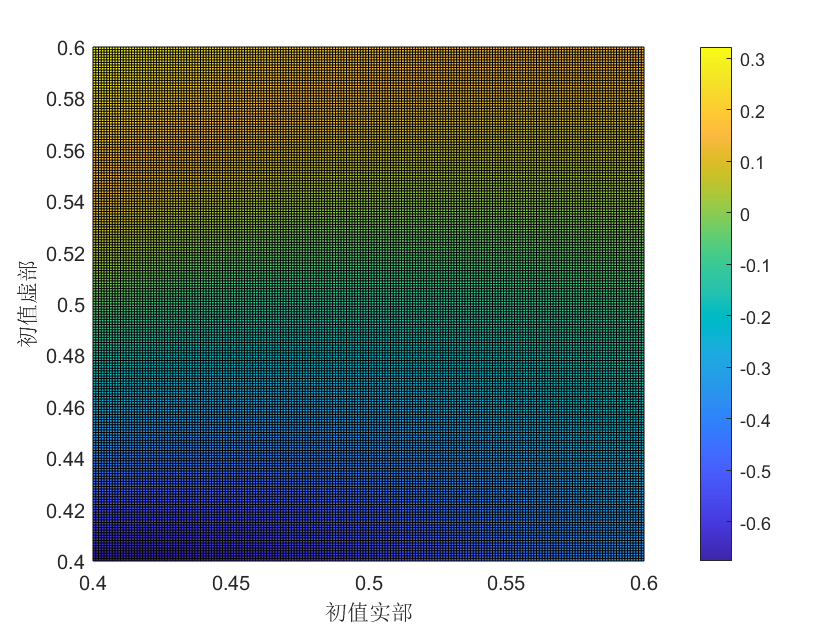
\includegraphics[scale=0.3]{pictures/2_2_2.png}
      \end{minipage}
     }
 \caption{虚部总体图(a)和俯视图(b)}}
 \label{2_2}
 \end{figure}

 \newline
	\begin{figure}[!htbp]
		\centering
		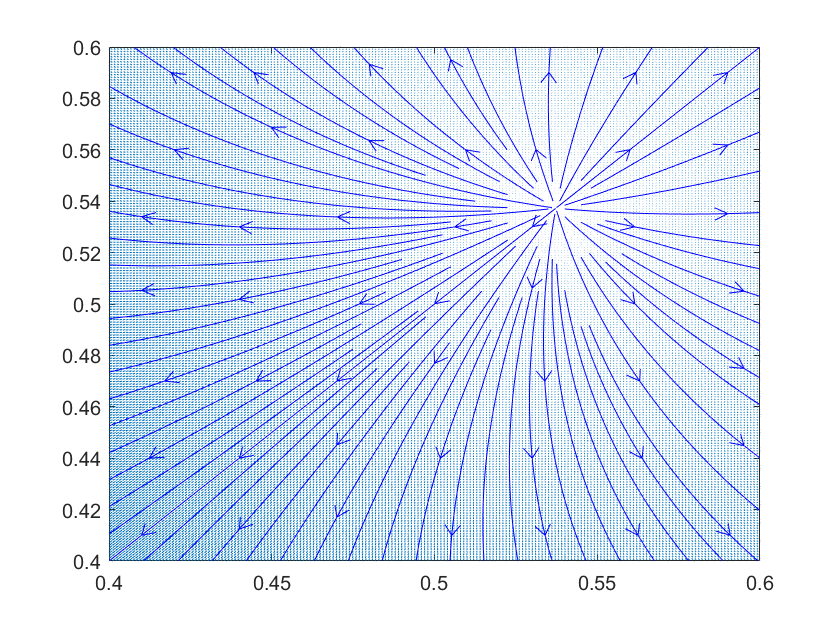
\includegraphics[width=1\textwidth,height=1\textwidth]{pictures/2_3.png}
		\caption{总体趋势图} \label{2_3}
	\end{figure}


\section{[0.49,0.51]\times [0.49,0.51],d=0.0001}
\subsubsection{代码展示}
~\\
\lstset{language=matlab}
\begin{lstlisting}
  %%
  %从不同初值z_{0}出发,用牛顿法求解复方程z^4=1的根
  clear;clc;
  R=0.49:0.0001:0.51;
  I=0.49:0.0001:0.51;
  newtonmethod(R,I)
\end{lstlisting}
\subsubsection{结果分析}
\newline
\begin{figure}[htbp]
  \centering
  \subfigure[]
  {
   \begin{minipage}{7cm}
    \centering
    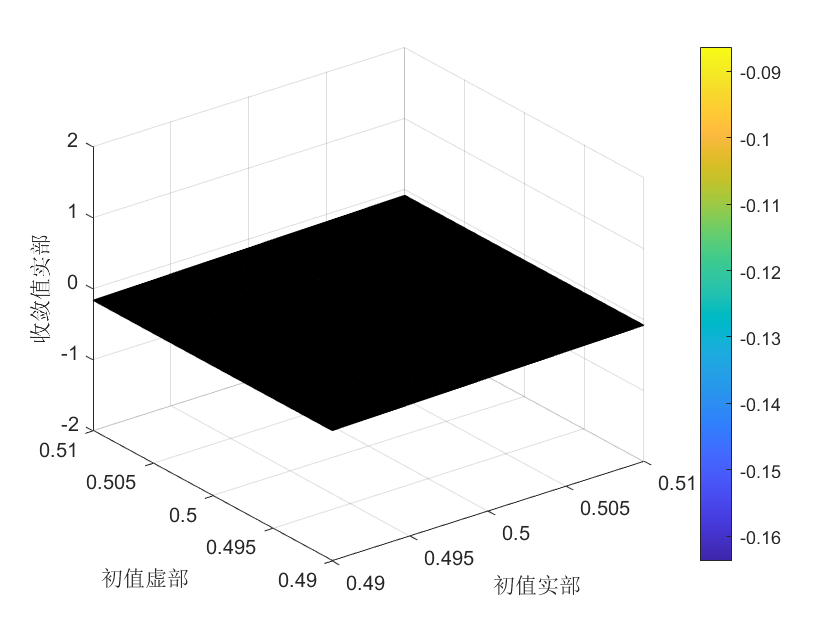
\includegraphics[scale=0.3]{pictures/3_1_1.png}
   \end{minipage}
  }
     \subfigure[]
     {
      \begin{minipage}{7cm}
       \centering
       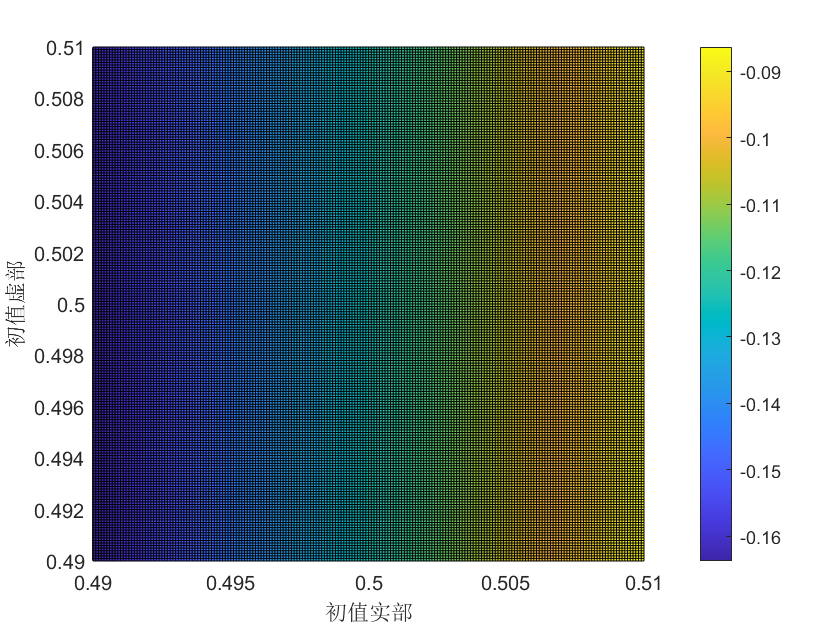
\includegraphics[scale=0.3]{pictures/3_1_2.png}
      \end{minipage}
     }
 \caption{实部总体图(a)和俯视图(b)}}
 \label{3_1}
\end{figure}

\newline
 \begin{figure}[htbp]
  \centering
  \subfigure[]
  {
   \begin{minipage}{7cm}
    \centering
    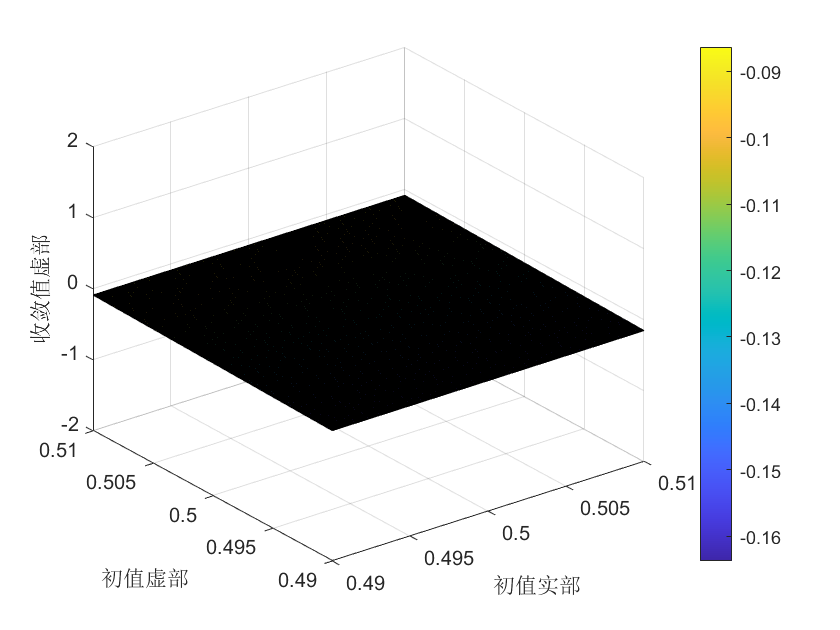
\includegraphics[scale=0.3]{pictures/3_2_1.png}
   \end{minipage}
  }
     \subfigure[]
     {
      \begin{minipage}{7cm}
       \centering
       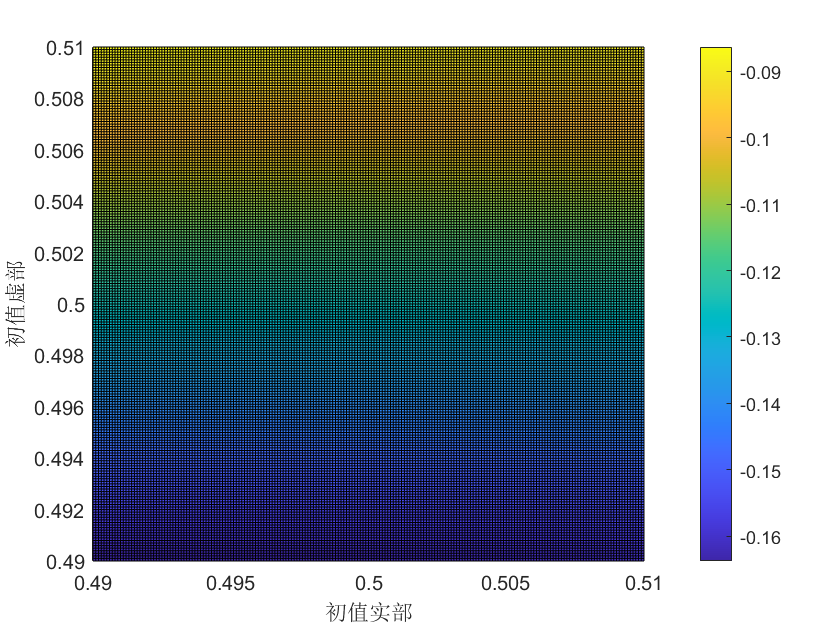
\includegraphics[scale=0.3]{pictures/3_2_2.png}
      \end{minipage}
     }
 \caption{虚部总体图(a)和俯视图(b)}}
 \label{3_2}
 \end{figure}

 \newline
	\begin{figure}[!htbp]
		\centering
		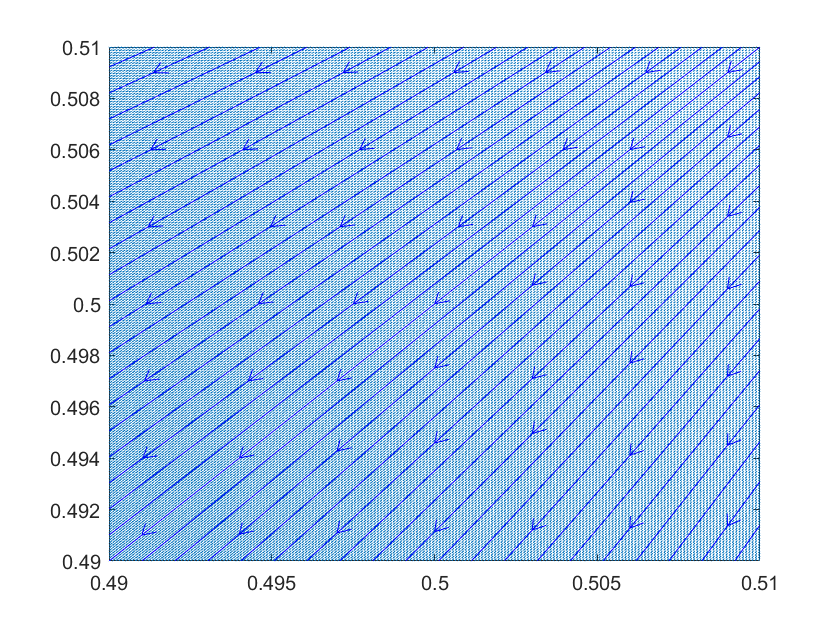
\includegraphics[width=1\textwidth,height=1\textwidth]{pictures/3_3.png}
		\caption{总体趋势图} \label{3_3}
	\end{figure}


\section{[0.499,0.501]\times [0.499,0.501],d=0.00001}
\subsubsection{代码展示}
~\\
\lstset{language=matlab}
\begin{lstlisting}
  %%
  %从不同初值z_{0}出发,用牛顿法求解复方程z^4=1的根
  clear;clc;
  R=0.499:0.00001:0.501;
  I=0.499:0.00001:0.501;
  newtonmethod(R,I)
\end{lstlisting}
\subsubsection{结果分析}
\newline
\begin{figure}[htbp]
  \centering
  \subfigure[]
  {
   \begin{minipage}{7cm}
    \centering
    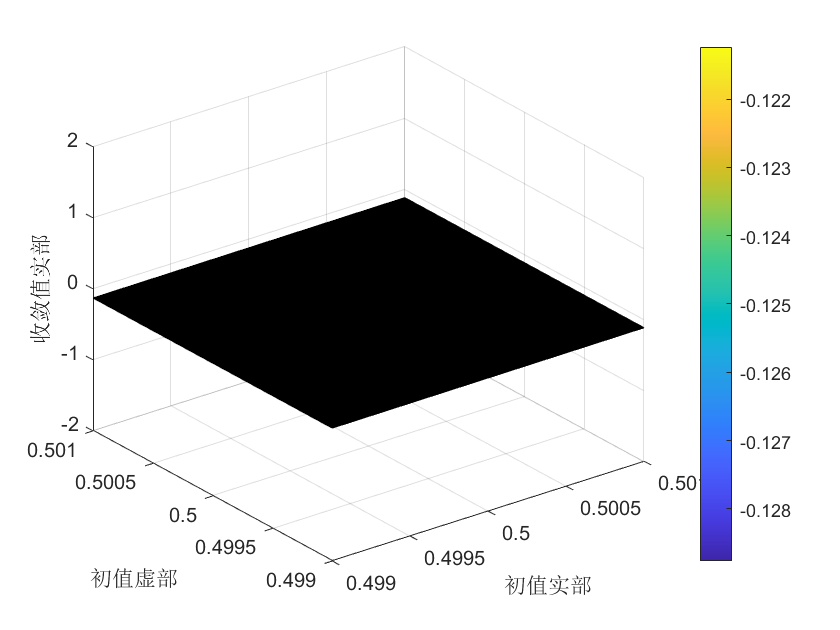
\includegraphics[scale=0.3]{pictures/4_1_1.png}
   \end{minipage}
  }
     \subfigure[]
     {
      \begin{minipage}{7cm}
       \centering
       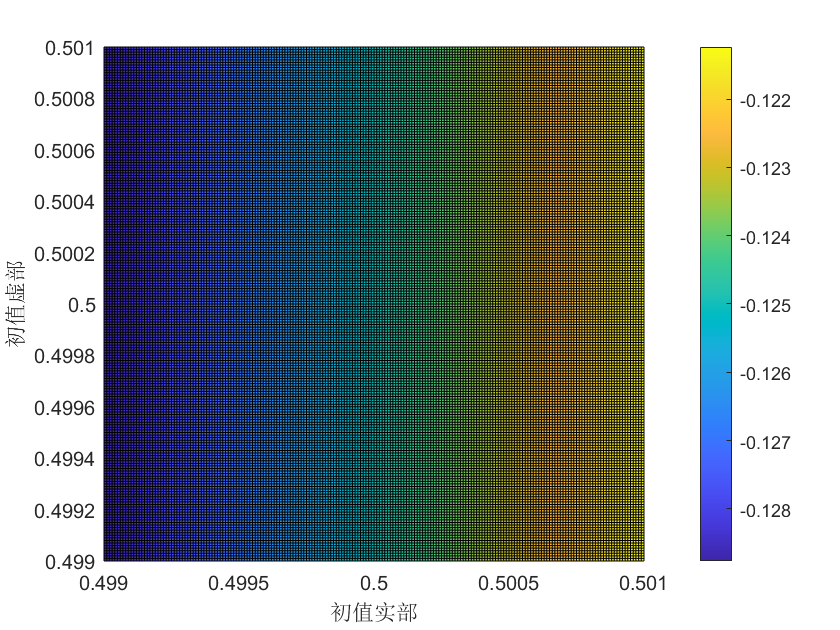
\includegraphics[scale=0.3]{pictures/4_1_2.png}
      \end{minipage}
     }
 \caption{实部总体图(a)和俯视图(b)}}
 \label{4_1}
\end{figure}

\newline
 \begin{figure}[htbp]
  \centering
  \subfigure[]
  {
   \begin{minipage}{7cm}
    \centering
    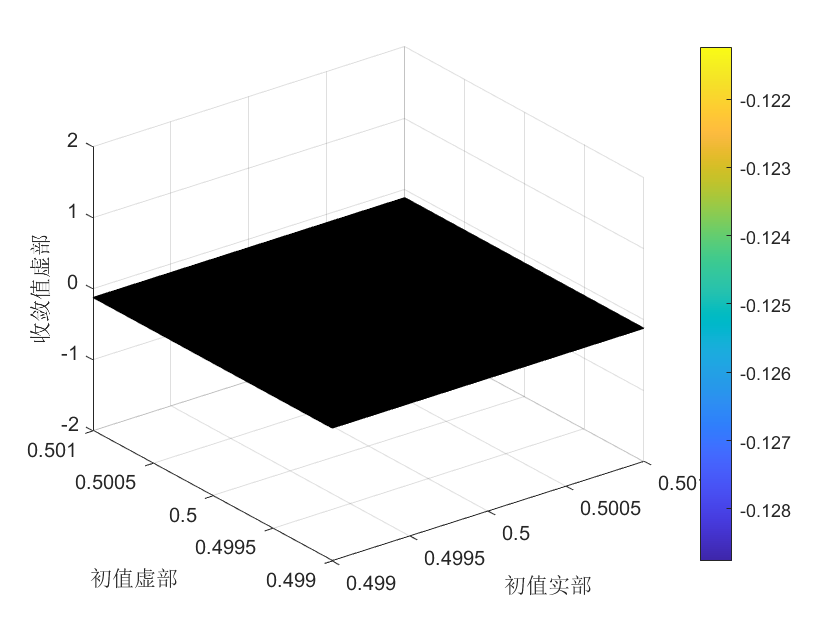
\includegraphics[scale=0.3]{pictures/4_2_1.png}
   \end{minipage}
  }
     \subfigure[]
     {
      \begin{minipage}{7cm}
       \centering
       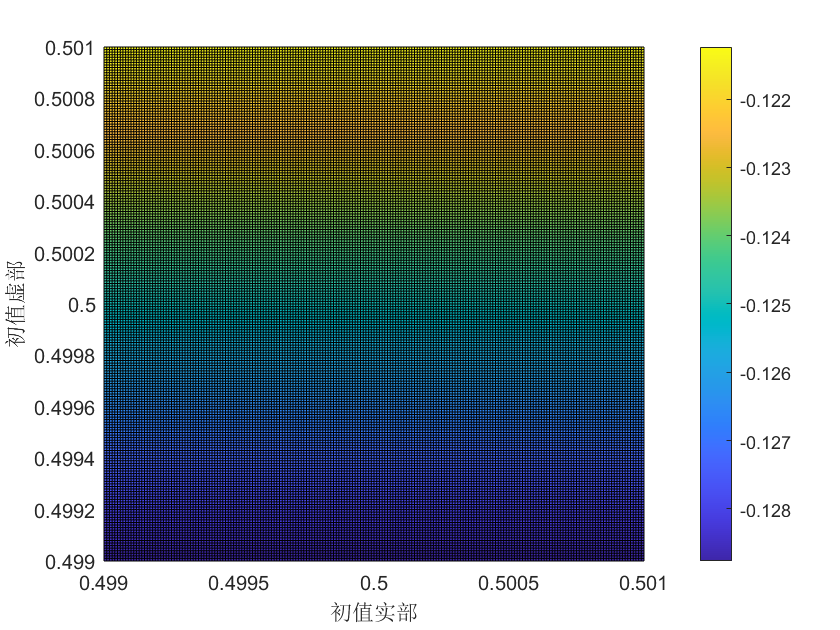
\includegraphics[scale=0.3]{pictures/4_2_2.png}
      \end{minipage}
     }
 \caption{实部总体图(a)和俯视图(b)}}
 \label{4_2}
 \end{figure}

 \newline
	\begin{figure}[!htbp]
		\centering
		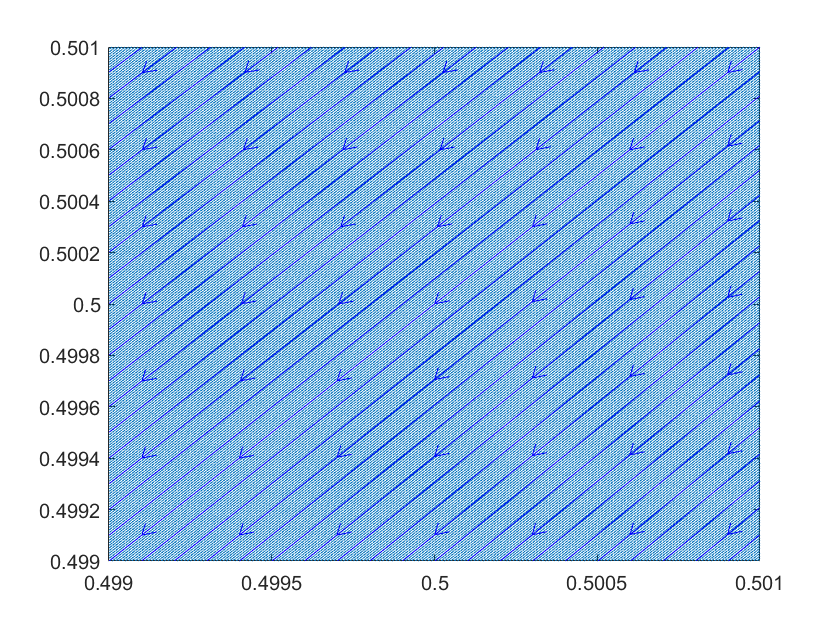
\includegraphics[width=1\textwidth,height=1\textwidth]{pictures/4_3.png}
		\caption{总体趋势图} \label{4_3}
	\end{figure}

  \section{图像分析与结论}
  由上述图像可知,随着扫描区域的缩小、扫描精细程度的提高,最后收敛的结果愈发得接近于同一个复数域内的值,
  且流线图随着上述过程越来越接近均匀场。由此可知,上述过程使得牛顿法对其的处理结果有明显的趋同过程。
%%%以下为插入图片模板
%\quad \newline
%	\begin{figure}[!htbp]
%		\centering
%		\includegraphics[width=0.5\textwidth,height=0.375\textwidth]{pictures/minscale.png}
%		\caption{最小风向} \label{minsacle}
%	\end{figure}

%%%以下为插入图片模板
%\quad \newline
%	\begin{figure}[!htbp]
%		\centering
%		\includegraphics[width=0.5\textwidth,height=0.375\textwidth]{pictures/minscale.png}
%		\caption{最小风向} \label{minsacle}
%	\end{figure}

%    \begin{algorithm}
%		\caption{Title of the Algorithm}
%     	\begin{algorithmic}[1]
%			\REQUIRE some words.  % this command shows "Input"
%			\ENSURE ~\\           % this command shows "Initialized"
%			some text goes here ... \\
%			\WHILE {\emph{not converged}}
%			\STATE ... \\  % line number at left side
%			\ENDWHILE
%			\RETURN this is the lat part.  % this command shows "Output"
%		\end{algorithmic}
%	\end{algorithm}

\end{document}